\subsection{Complex systems}
\label{sec:characteristics}
%“Summary: What are complex systems”
Complex systems are those where many similar parts interact with each other using simple rules to create the whole,
which exhibit characteristics different than the parts --
``more is different''~\citep{anderson1972}.
Complex systems contrast with complicated systems, where many different parts with defined roles are put together to create the system. 
Complicated systems, such a watch, can be studied by analyzing their parts. 
Moreover the failure of a piece produces the failure of the system.
Complex systems, such a bird flock, cannot be studying by analyzing only their parts, 
but the interactions among them are also needed.  
Although a consensus definition of complex system does not yet exist, a complex system is characterized by the following attributes. 
1. Multi-scale: Many individual parts interact to create the whole. 
2. Networks: The individuals usually interact with a few other individuals, creating a network of interactions. For social systems, the networks created are ``small-world'' networks, where the distance between two random people in a network is small.  
3. Emergent properties: The whole has properties that none of the individuals have. 
4. Spontaneous order. There is not a global organizer of the system. For instance, the standing ovation is an emergent property of the interaction between people. 
5. Memory: The individuals remember previous interactions. 
6. Feedback loops: The interaction between two individuals affect other individuals in the system. For example your decision about standing up affects the probability that other people start standing up.  
7. Stochasticity: The system lives in a noisy environment. 
8. Steady-states are far from equilibrium. Complex systems are usually in a steady-state (except during transition times). However, since they depends on active interactions between people, they stay far from the equilibrium. If no energy is added to the system, the system disappears.
9. Non-linearity, cascading and hysteresis. The interactions are non additive. For the standing ovation, the addition of a new person standing can produce a cascade of events.
10. Robustness to random failures. The system is highly resistant to the failure of one of the individuals. 
11. Sensitivity to targeted failures if individuals are organized in network: The system is sensitive to the failure/removal of a few specific individuals. 

\subsection{The micro-macro problem}
%“Summary: Interactions are important”
Some social systems exhibit different properties than the parts composing them.
In those systems, the action of an agent cannot be solely predicted from its characteristics, 
but the interactions between agents need to be taken into account. 
For instance, it is more likely that you start using purple hats if your partner thinks that are trendy than if your colleague does,
which in turn affect the probability of your friends and colleagues also wearing purple hats.
The probability that every person in society start using purple hats cannot be predicted by their perceived trendiness, 
but networks must be taken into account.
Similarly, the performance of a firm depends not only on their product,
but also on the interaction between firms, governments and other groups, 
which in turn are composed and influenced by individuals.
Moreover, the success of their product 
-- which is partly based on the interaction with other firms and groups -- 
affects the actions of your suppliers and competitors.
A classic example are format wars,
where inferior products can (and often do) succeed.
The problem where the whole depends on both the parts and the interaction between pars is often called `the micro-macro problem'.

%“Summary: The whole is different than the sum of the parts”
The micro-macro problem is found across disciplines. 
In physics, snowflakes form by the interaction between low-energy $H_20$ molecules, 
where the specific shape of the flake depends on the interactions between the individual molecules.
In biology, organs are composed of individual cells that do not have the properties of the organ. 
A cardiac cell alone lack the capability to beat, however a few hundreds of cells together spontaneously start to beat.
In ecology, ant colonies are efficiently organized to collect food, clean and defend the colony, and reproduce. 
However an individual ant cannot perform all those tasks, 
but requires chemical stimuli from other ants to coordinate.
In social systems, complex behaviours are the results of the interactions between the agents. 
A mediocre play can receive a standing ovation if a group stands up immediately after the play ends, 
creating a cascade of people standing up~\citep{miller2004}. 

Importantly, although predicting the whole in individual situations is difficult, 
this does not imply that we cannot observe correlations at the macro scale. 
In our physics example, humidity and temperature increase the probability of a specific shape of the snowflake. 
Cardiac cells will be more likely to beat if specific chemicals are added.
A colony of ants will be more likely to leave the colony to scavenge for food if the temperature is low. 
A play will be more likely to receive a standing ovation example if it is good.
However, it is important to observe that the correlations are indirect.
The humidity does not affect the shape directly, but affect the probability of two molecules of water binding in an specific way. 
The quality of the play will increase the probability that some people stands up, 
creating a cascade of people standing. 
Because macro outcomes are non-linear aggregations of the micro agents, 
an appropriate model for the micro-macro problem is required.
%It is important noting that ``rare events'' in complex systems,
%such as heart attacks, ecological disasters, or key events in history, 
%are caused by cascades of events originated by random events,
%and thus causality is tricky


\subsection{The micro-macro problem in social sciences. A complex systems perspective}
\label{sec:complexSocialSystems}
\begin{figure}[h!]
\begin{center}
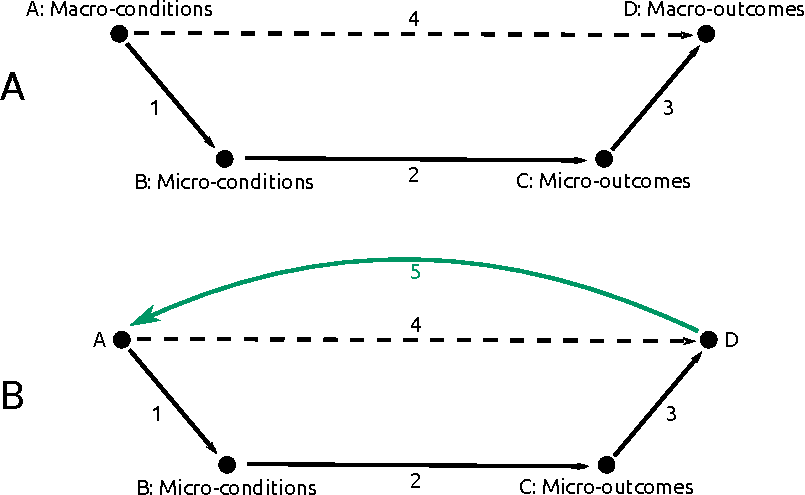
\includegraphics[width=.5\textwidth]{coleman.pdf}
\end{center}
\caption{Global network of interlocking directorates. Color indicates communities -- i.e. cities that do business together within each other more often than with others. Adapted from \cite{raub2011micro}}
\label{fig:coleman_scheme}
\end{figure}

%“Summary: Being able to think doesn’t really make you so special in the eyes of the Complexity Deity”
In social sicences, Colleman’s scheme~\citep{coleman1990} (Fig.~\ref{fig:coleman_scheme}A) is the standard framework to represent the micro-macro problem.
Nodes A and D in Figure.~\ref{fig:coleman_scheme} are the macro-conditions (composed of the environment where the system is situated) and macro-outcomes of the social system. 
Node B corresponds to the micro-conditions (composed of the perceived environment, as well as genetic and other individual factors). 
Micro-conditions are affected by the macro-conditions. 
This arrow is usually labeled as bridge assumptions.
Micro-outcomes are the decisions of the individual among the possible options. 
In the standing ovation example, this corresponds to each individual decision to stand up or not. 
This arrow is non-trivial, since the decision does not depend only on each agent's conditions, 
but also on interdependent relationships with other individuals.
In Granovetter's model~\cite{granovetter1978}, the individuals are characterized by a threshold $\phi$ that summarizes their micro-conditions. 
Each person will then riot if there are at least $\phi$ other people rioting already.
Similarly to the standing ovation, the population will end up in a generalized revolution, 
or it will die off depending on the distribution of thresholds in the population. 
For instance, consider population A, where 10\% of a population starts rioting, but the other 90\% will not riot unless 20\% of the population is rioting.
In this population, the `average' person will riot if 18\% of the population are rioting, but no revolution will occur.
Imagine now population B, where 10\% of the population starts rioting, another 20\% will riot if 10\% is already rioting and the final 70\% will only riot if 30\% of the population is rioting the revolution will spread. 
In population B, the `average' person will riot if 23\% are already rioting, however due to the non-linearity in the aggregation a revolution will occur.
The aggregation of the micro-outcomes (the individual decisions to riot or not riot) corresponds to label 3. This arrow is usually labeled as transformation rules.


%“Summary: it is a cycle you dumb”
Coleman’s original scheme~\cite{coleman1990} uses Webber’s origin of capitalism~\citep{weber1904} as an example, 
linking it to the micro-macro problem. 
He explains the rise of capitalism (D) from protestant religious doctrine (A). 
A protestant religious doctrine creates specific values in the individuals (B) that produce certain economic behaviours (C). 
The aggregation of these economic behaviours gives rise to the capitalism (D). 
Capitalism is the result of the economic behaviour of people, which in turn is caused by the individual interpretation of the values of protestantism.
A revolution is the result of the decision of people to riot given their angriness level caused by the macro-conditions.
While apparently coherent, this reasoning has two main flaws, 
Firstly, it obviates the link from (D) to (A). 
The origin of capitalism was a process that lasted decades, 
where the economic behaviours produced some intermediate macro-outcomes that affected the macro-conditions. 
This in turn affects the micro-conditions (values), 
which affect the micro-outcomes (economic behaviour) from the previous time point. 
Capitalism is one of the steady states of the cycle.
Our view of the process, using Granovetter model as an example, is summarized in Figure~\ref{fig:coleman_scheme}B. 
In Granovetter example there are some specific macro-conditions at time zero, 
such as a level of hunger, a level of police reprisal, or a sense of collective.
Moreover, no people are rioting ($\Phi_0 = 0$, where $\Phi_0$ is the percentage of the population rioting at time 0). 
Given the micro-conditions, a few people ($x$) with threshold zero ($\phi_i == 0 \geq Phi_0$) -- very prone to riot -- make the individual decision to riot (micro-outcome). 
The macro-outcome is that a group of people are rioting. 
This affects the macro-conditions ($\Phi_1 = x$). 
The micro-conditions in Granovetter model are fixed (constant thresholds, although this is a simplification).
Now, every individual compares their own threshold with $\Phi_1$, and riot if $\phi_i \geq Phi_1$. 
The cycle continues until we reach a stable state (for example revolution or just a few people rioting).
This class of systems where the system is continuously evolving correspond to Complex Adaptive Systems.


%“Summary: adding a bit of complex systems ”
The second flaw is that it creates an illusion of determinism.
In any complex system, random events can create a cascade of events that cannot be explained solely by the macro-conditions. 
Furthermore, we can always find a logical explanation of the end result.
For instance, we can deduct that that few people started rioting because police reprisal, and that produced the cascade.
However these kind of `ad hoc' explanations makes police reprisal a necessary condition, 
while the same could have happened with no police reprisal, 
or no rioting could have happened with the same reprisal.
While we could probably say that some degree of police reprisal increased the propensity of rioting,
we cannot conclude that reprisal is a necessary cause of rioting,
or that police reprisal will cause another revolution in similar conditions.
When the end result is the non-linear aggregation of many interconnected actors,
the results can only be generalized
when we can compare many independent, similar cases~\citep{watts2007}.


%“Summary: Complex system research is cooool”
In the past decades we have seen the recollection of large datasets for many complex systems. 
These large dataset include vast information on biology (e.g. interactions between thousands of proteins in the cell),
social interactions (e.g. social networks, movement trackers, etc),
or the economy (e.g. Orbis, Reuters or LexisNexis provide information on firm indicators and directors for millions of companies worldwide).
As a consequence, new methods and models have been developed for the study of these rich datasets. 
These tools can be grouped in three categories.
1. Descriptive tools: To characterize the macro-outcomes and find patterns in the data.
2. Generative modelling: To explain emergence of macro-outcomes from the micro scale, how the macro-conditions affect the micro scale, or both.
3. Predictive tools: A model is useful if it provide insights in the causal mechanisms and can predict future events. This include predicting what has already happened using only a portion of the data. 
An example that combines the three categories is the work that resulted in the Atlas of Economic Complexity and that will be the basis of next section~\citep{Hausmann2006,hidalgo2007,hidalgo2009,hausmann2011}.
Firstly, they described every country (macro scale) with respect to the type and amount of exports and imports (micro scale). 
Secondly, they assumed a series of capabilities required to produce a product (for example institutions, materials, human capital). 
If countries produce the products when they acquire the capabilities required to produce it, 
then products that are often exported together will require similar capabilities.
Since it is not possible to quantify those capabilities, they created the one-mode projection of the model,
namely network of products (named the `product space'), where two products were closer in the network if they were usually exported together. 
Thirdly, they modeled the development of countries, showing that countries develop by acquiring new capabilities and producing products that are close in the product space.
For instance, a country may develop an electronic industry if they chemicals is an important export, 
but not if they rely on exporting cereals~\citep{hidalgo2007}. 
Finally, they used the current products produced in the country to create a better indicator for the economic growth of the country~\citep{hausmann2011}.
Linking back to Coleman’s modified scheme (Fig.~\ref{fig:coleman_scheme}B) we see how the products that a country currently export and import (macro-conditions at time zero) affect the products that companies can produce (micro-conditions at time zero). 
This in turn affect the products that they actually produce (micro-outcomes at time zero), 
which results in the total exports and imports (macro-outcomes at time zero).
In this model, the macro-outcomes at time zero correspond to the macro-conditions at time one. 
Understanding the cycle has utility to focus investment on certain sectors.


\subsection{Complex system toolbox for network analysis}
We next (very) briefly summarize general methods to study data in complex systems.
Because most social and economical systems are embedded in networks, we will focus on complex networks. 
The standard notation treats networks (graphs) as a series of nodes and edges, where nodes are the agents and edges the interactions between agents.


\subsubsection{Descriptive tools}
Descriptive tools are used to find patterns in the data.
Summary statistics, correlations and visualizations allow for a rapid exploration of the data, and an assessment of data quality.
Two of the main tools are community detection and centrality analysis.
Community detection finds nodes that interact with each other more than with the rest of the network.
For example in a recent paper we studied a network of firm interlocks (ref), 
where the nodes correspond to firms and the edges to shared directors.
We showed that in some regions the business communities are organized along national borders, 
whereas in other areas the locus of organization is at the city level or international level. 
Centrality analysis grades the importance of a node in the network. 
Different centrality measures have been developed. 
For instance in betweenness centrality a node is important if it connects far regions in the network. 
The specific measure will depend on the problem. 
If we are measuring the spread of information, 
as Granovetter did in the strength of weak ties~\citep{Granovetter1973}, 
betweenness centrality would be indicated.


Communities and centralities have been used abundantly to describe data.
In Clauset et. al.~\citep{Clauset2015} description of inequality in academia, 
they mapped the academic trajectory of 19,000 faculty in three disciplines.
From the mapping, they rank each institution by its relative ``prestige centrality''.
Institution A is more prestigious than B if people can do their PhD in A and move to B, 
but PhD graduates from B cannot find a job in A.
They showed that the top 25\% of the institutions positioned 71-86\% of all tenure-track faculty,
revealing steep inequality and clear hierarchical networks.



\subsubsection{Modeling}
Modeling allows us to understand the world and predict future events better than people~\citep{tetlock2005} .
For example, modeling the network of bank co-risk (Fig. \ref{fig:corisk}) allowed authorities to assess the risk of not bailing out banks.
The end result was the bankrupcy of Lehman Brothers and the bailing out of AIG.
The goals of modeling are to make causal inferences about a phenomenon and to predict future events.
Three main models are used:
Firstly, traditional statistical models explains an independent variable in terms of dependent variables. 
They are characterized by a formula whose parameters are estimated.
The parameters usually have a direct real-life interpretation.
They emphasize inference and work well when the number of dependent variables is small.
The most common example of the group is regression.
Secondly, machine learning are also used to explain the results of an output (our dependent variable) in terms of an input (independent variables).
Opposing statistical models, they are usually black-boxes, meaning that real-life interpretation of the weights do not exist.
Consequently, they emphasize prediction and are used when the number of dependent variables is large (big data).
Finally, mathematical and computational modeling allows to recreate the physical system and understand the causes that drive the output of the system.



\begin{figure}[h!]
\begin{center}
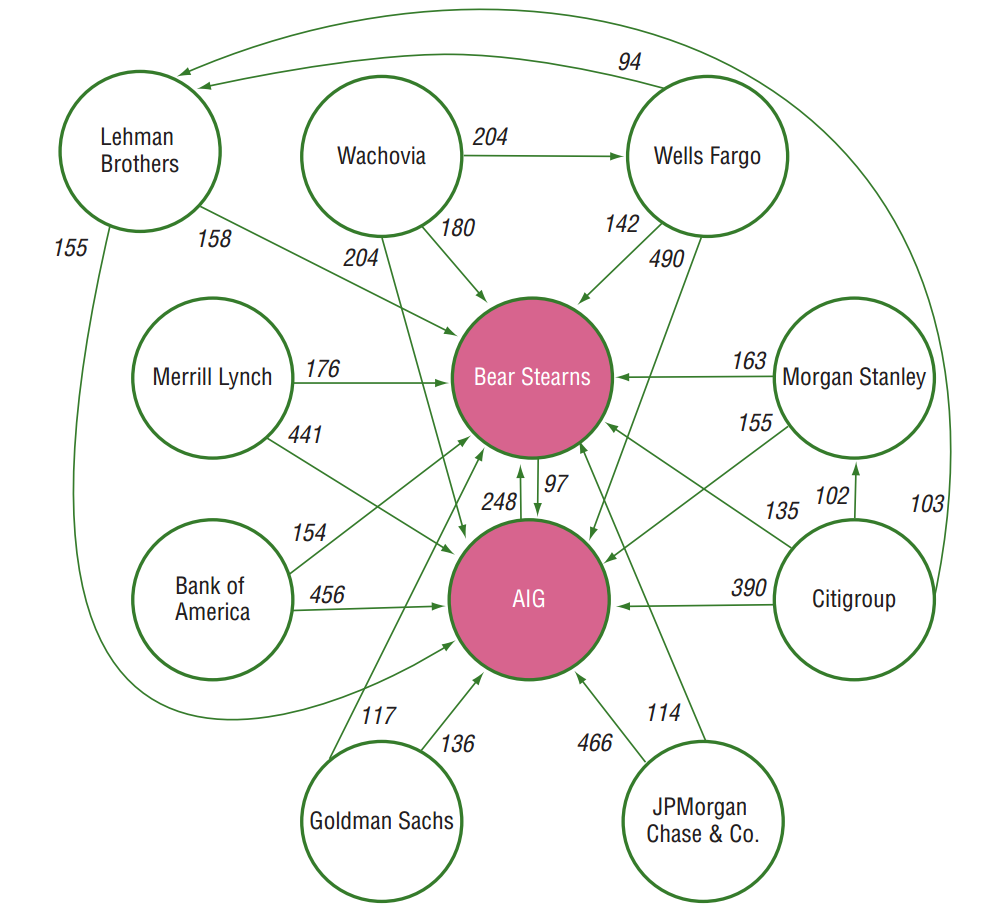
\includegraphics[width=.5\textwidth]{corisk.png}
\end{center}
\caption{Sources: Bloomberg, L.P.; Primark Datastream; and IMF staff estimates.
Note: This figure presents the conditional co-risk estimates between pairs of selected financial
institutions. Only co-risk estimates above or equal to 90 percent are depicted. See Table 2.6 for further
information.~\citep{corisk2009}}
\label{fig:corisk}
\end{figure}


\textit{Mathematical and computational modeling}

As previously discussed, it is not possible to explain emergent properties just by studying the agents.
Mathematical and computational models allow to close the gap between the micro and macro scales.
In Granovetter rioting example, a mathematical model allows us to understand why a population will end up rioting, while other more prone to riot on average will not.
In the segregation example of Schelling~\citep{schelling2006}, 
a neighborhood of houses is simulated in a square lattice (chess board), 
where most houses are occupied but some are empty, 
allowing the inhabitants to move between houses.
Two different types of person live in the houses (let’s call them Belgians and Dutchies) in equal proportion.
None of them are racists, but they would like to have at least two neighboors that are like them.
If they do not have at least 25\% of the neighbors that are like them they move at random to one of the empty houses. 
While the at random will not hold in reality, it is a conservative scenario.
If segregation is found with this simple model, selectively moving to neighbourhoods with a large population of your kind will only produce higher segregation rates.
The result is the clear segregation showed in Figure \ref{fig:seggregation}A , that resembled the segregation in life (Fig. \ref{fig:seggregation}).


\begin{figure*}
\begin{center}
\includegraphics[width=.95\textwidth]{seggregation.pdf}
\caption{Gwhite is pink (heavier concentrations look reddish), black is blue, Hispanic is orange, and Asian is green..}
\label{fig:seggregation}
\end{center}
\end{figure*}



Mathematical and computational models can help us discover how simple rules can produce complex macro results. 
Models can be classified in several categories. 
According to their assortativity, they are classified into 
perfect mixing models, where all the agents can interact with all other agents,
and network models, where the agents can only interact with a subset of other agents.
According to the presence of noise they can be classified into
deterministic and stochastic, where some amount of noise is included.

According to the method used to solve the model, they can be classified into
equation-based models (analytical and numeric), where the population is represented with an equation,
and agent-based models, where each individual is modeled individually (see Epstein~\citep{Epstein2006} for an excellent review and implications of agent-based models in social sciences).
The type of model will depend on the application.
For example if we want to measure the effect of time and distance on terrorist attacks,
using an analytical model (Hawkes process), where an attack produces a cascade of events, will be useful~\citep{garciab2015}.
If you are interested on modeling smoking behavior in high schools,
an agent-based model that includes selection and influence terms may be more appropriate~\citep{Mercken2010}.


In political sciences, such models have been successfully applied to understand the spreading of ideas (contagion such as granovveter, Generalized contagion models (Dodds and Wattas 2004,2005): memory of exposure to a contagious entity (e.g. a rumor or disease), variable magnitudes of exposure (dose sizes), and heterogeneity in the susceptibility of individuals), 
to understand the factors affecting polarization vs homogenization. 
to find the micro-motives in the origin of inequality, 
show why coordination and collaboration emerge,
among others (refs for all). 
In general, modeling allows us to find and quantify which micro and macro-conditions are associated to the macro-outcomes observed.




%Two important parts that many models dealing with social interactions are preferential attachment and clustering of similars. 
%Preferential attachment is the tendency of popular/rich agents get more popular/rich, 
%which creating fat tail distributions.
%This phenomenon is intrinsically related to inequality, but affect any network.
%Clustering of similars correspond to the increased interaction between similar people. 
%For instance, xx and yy (ref) showed that people who smoke are usually friends with people that also smoke.
%Two mechanisms can explain this.
%The first is selection (assortativity/homophily).
%You use to choose friends that smoke, for example by going out to smoke in every work break.
%The second mechanism is influence (contagion).
%You influence (or are influenced by) your friends to smoke.
%The two mechanisms result in the same macro-outcome, similar people interacting together.
%The distinction between these two mechanism is only possible when longitudinal data is available. 
%If the mechanism is selection most people in the group should smoke from the moment that the link is created.
%However if the mechanism is influence people will start smoking after the link is created.
%Correcting and understanding preferential attachment and clustering of similar is key when modeling real systems.

%For a review on sociological explanations for dyadic formation: see~\cite{Rivera2010}

%The MLE with the so-called Miller-Madow bias correction (Miller,
%1955),
%HˆMM(pN) ≡ HˆMLE(pN) +
%mˆ − 1
%2N ,
%he maximum likelihood (ML) estimator given pN (also called the
%“plug-in”—by Antos & Kontoyiannis, 2001) or “naive”—by Strong et
%al., 1998—estimator),
%
%HˆMLE(pN) ≡ −m
%i=1
%pN,i log pN,i


\subsubsection{Prediction}
Modeling alone . 

For this reason, prediction capabilities are often required.

Another way to 

null models

Epstein reference

\subsection{Summing up}
Social science systems are often embedded in complex networks of interconnected agents, 
where the action of an agent affect the actions of the others in a non-linear fashion.
With the advances in technology, 
we are for the first time able to gather large datasets of social systems.
Data availability has come together intensive research in the area of complex systems,
and we have now models to describe, model and predict these challenging structures.


